\chapter{Full Imitator code of the hammer example}

{\small
\begin{verbatim}
var
      session, t
           :clock;


      sessionTime,
      reactTime
           : parameter;


      nails
           : discrete;


      totalNails = 20
        : constant;




automaton Worker


synclabs: rest, hit, newNail, Work;

loc Rest: invariant session <= sessionTime - reactTime
      when True sync Work do {t := 0} goto Work;

loc Work: invariant session <= sessionTime && t <= reactTime
      when t >= reactTime sync newNail do {t := 0} goto Work;
      when t >= reactTime - 5 sync hit do {t := 0} goto Work;
      when session >= sessionTime sync rest do {session := 0} goto Rest;

end



automaton Hammer

synclabs: hit, newNail;

loc NailUp: invariant True
      when True sync hit goto NailHalf;

loc NailHalf: invariant True
      when countNails = True sync hit do {nails := nails +1} goto NailDone;

loc NailDone: invariant True
      when infiniteNails = True || nails <= totalNails sync newNail sync newNail goto Nailup;

end


init := 


        & loc[Worker] = Rest
        & loc[Hammer] = NailUp


        & session = 0
        & t = 0

    & nails = 0

    & sessionTime >= 0
    & reactTime >= 0


;


end
\end{verbatim}
}

\chapter{Running Imitator with the hammer example}

%explicar a secção

\begin{verbatim}
    
------------------------------------------------------------
Number of IPTAs                         : 2
Number of clocks                        : 2
Has invariants?                         : true
Has clocks with rate <>1?               : false
L/U subclass                            : U-PTA
Bounded parameters?                     : false
Has silent actions?                     : false
Is strongly deterministic?              : true
Number of parameters                    : 1
Number of discrete variables            : 1
Number of actions                       : 4
Total number of locations               : 5
Average locations per IPTA              : 2.5
Total number of transitions             : 7
Average transitions per IPTA            : 3.5
------------------------------------------------------------
\end{verbatim}

\begin{tcolorbox}[colframe=red]
\begin{verbatim}
BEGIN CONSTRAINT
 Parameter Constrain
END CONSTRAINT
\end{verbatim}
\end{tcolorbox}

\begin{verbatim}
------------------------------------------------------------
Constraint soundness                    : exact
Termination                             : regular termination
Constraint nature                       : good
------------------------------------------------------------
Number of states                        : 1
Number of transitions                   : 0
Number of computed states               : 2
Total computation time                  : 0.007 second
States/second in state space            : 128.6 (1/0.007 second)
Computed states/second                  : 257.2 (2/0.007 second)
Estimated memory                        : 2.078 MiB (i.e., 272498 words of size 8)
------------------------------------------------------------

------------------------------------------------------------
 Statistics: Algorithm counters
------------------------------------------------------------
main algorithm + parsing                : 0.043 second
main algorithm                          : 0.014 second
------------------------------------------------------------
 Statistics: Parsing counters
------------------------------------------------------------
model parsing and converting            : 0.025 second
------------------------------------------------------------
 Statistics: State computation counters
------------------------------------------------------------
number of state comparisons             : 0
number of constraints comparisons       : 0
number of new states <= old             : 0
number of new states >= old             : 0
StateSpace.merging attempts             : 0
StateSpace.merges                       : 0
------------------------------------------------------------
 Statistics: Graphics-related counters
------------------------------------------------------------
state space drawing                     : 0.000 second
------------------------------------------------------------
 Statistics: Global counter
------------------------------------------------------------
total                                   : 0.050 second
\end{verbatim}

\chapter{Uppex HTML Coffee Result}

\begin{figure}[H]
    \centering
    \begin{minipage}{\textwidth}
        \centering
        \begin{tikzpicture}
            \node[anchor=south west,inner sep=0] (image1) at (0,0) {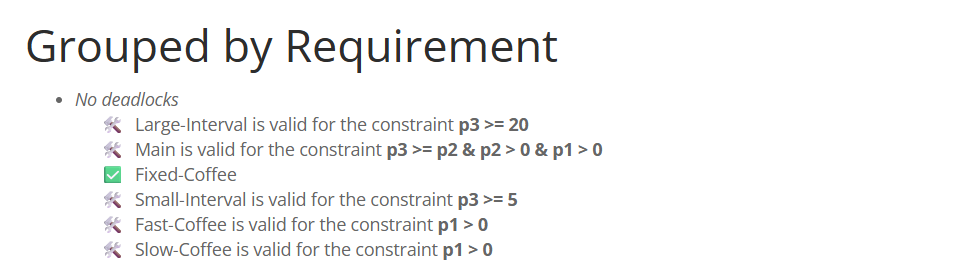
\includegraphics[width=\linewidth]{images/fixed_end.png}};
            \begin{scope}[x={(image1.south east)},y={(image1.north west)}]
                \draw[black, thick] (0,0) rectangle (1,1); % coordenadas normalizadas
            \end{scope}
        \end{tikzpicture}
        \caption{Grouped by Requerimets Report Result}
        \label{fig:Fixed_C}
    \end{minipage}
\end{figure}

\begin{figure}[H]
    \centering
    \begin{minipage}{\textwidth}
        \centering
        \begin{tikzpicture}
            \node[anchor=south west,inner sep=0] (image1) at (0,0) {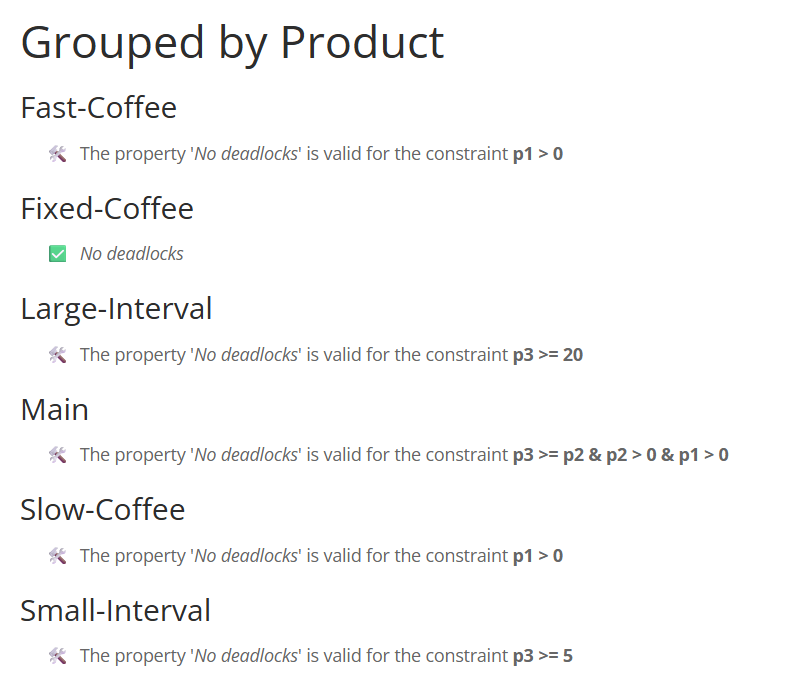
\includegraphics[width=\linewidth]{images/Grouped.png}};
            \begin{scope}[x={(image1.south east)},y={(image1.north west)}]
                \draw[black, thick] (0,0) rectangle (1,1); % coordenadas normalizadas
            \end{scope}
        \end{tikzpicture}
        \caption{Grouped by Requerimets Report Result}
        \label{fig:Fixed_G}
    \end{minipage}
\end{figure}

\begin{figure}[H]
    \centering
    \begin{minipage}{\textwidth}
        \centering
        \begin{tikzpicture}
            \node[anchor=south west,inner sep=0] (image1) at (0,0) {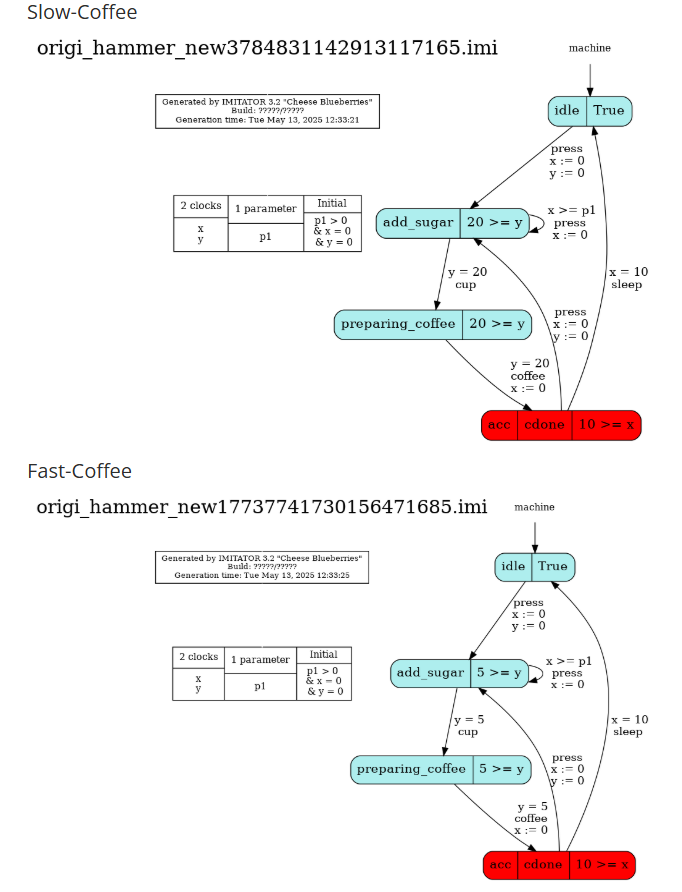
\includegraphics[width=\linewidth]{images/im1.png}};
            \begin{scope}[x={(image1.south east)},y={(image1.north west)}]
                \draw[black, thick] (0,0) rectangle (1,1); % coordenadas normalizadas
            \end{scope}
        \end{tikzpicture}
        \caption{Coffee Automata Products Part 1 Report Result}
        \label{fig:Fixed_im1}
    \end{minipage}
\end{figure}

\begin{figure}[H]
    \centering
    \begin{minipage}{\textwidth}
        \centering
        \begin{tikzpicture}
            \node[anchor=south west,inner sep=0] (image1) at (0,0) {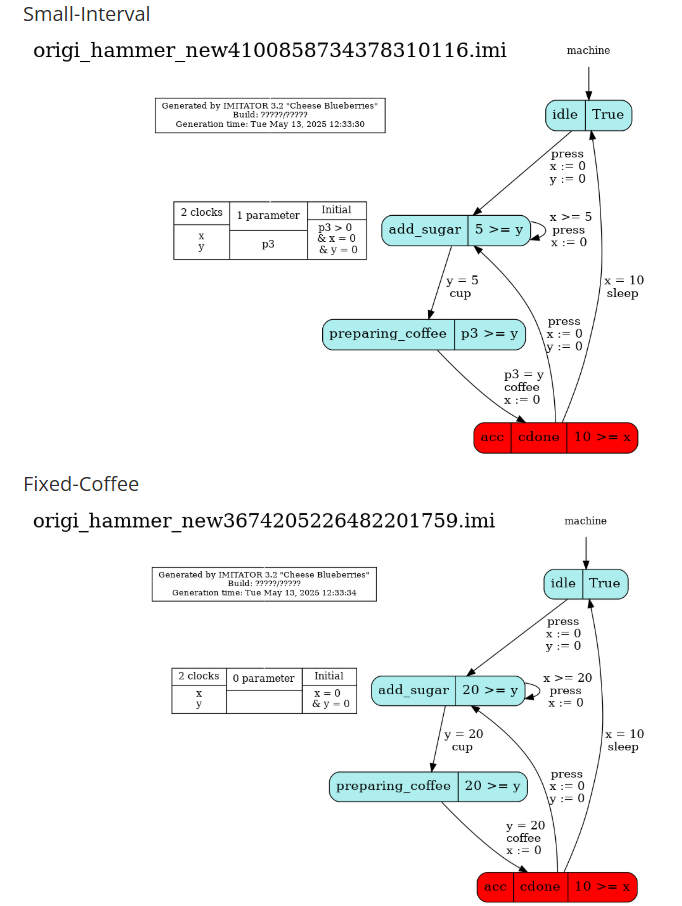
\includegraphics[width=\linewidth]{images/im2.png}};
            \begin{scope}[x={(image1.south east)},y={(image1.north west)}]
                \draw[black, thick] (0,0) rectangle (1,1); % coordenadas normalizadas
            \end{scope}
        \end{tikzpicture}
        \caption{Coffee Automata Products Part 2 Report Result}
        \label{fig:Fixed_im2}
    \end{minipage}
\end{figure}

\begin{figure}[H]
    \centering
    \begin{minipage}{\textwidth}
        \centering
        \begin{tikzpicture}
            \node[anchor=south west,inner sep=0] (image1) at (0,0) {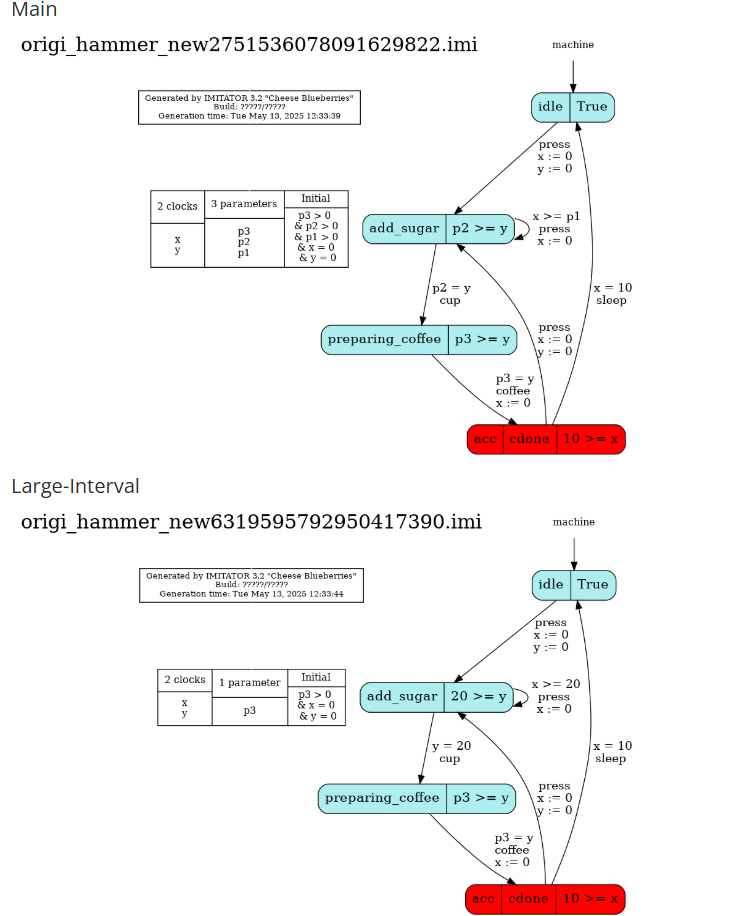
\includegraphics[width=\linewidth]{images/im3.png}};
            \begin{scope}[x={(image1.south east)},y={(image1.north west)}]
                \draw[black, thick] (0,0) rectangle (1,1); % coordenadas normalizadas
            \end{scope}
        \end{tikzpicture}
        \caption{Coffee Automata Products Part 3 Report Result}
        \label{fig:Fixed_im3}
    \end{minipage}
\end{figure}


\chapter{Uppex HTML Hammer Result}
%colocar link

\begin{figure}[H]
    \centering
    \begin{minipage}{\textwidth}
        \centering
        \begin{tikzpicture}
            \node[anchor=south west,inner sep=0] (image1) at (0,0) {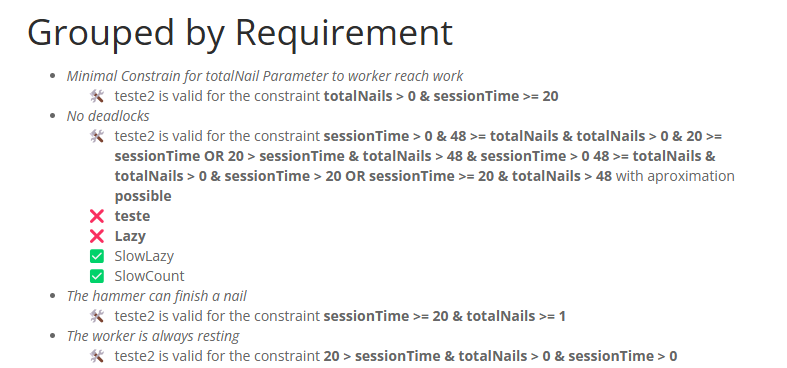
\includegraphics[width=\linewidth]{images/res1.png}};
            \begin{scope}[x={(image1.south east)},y={(image1.north west)}]
                \draw[black, thick] (0,0) rectangle (1,1); % coordenadas normalizadas
            \end{scope}
        \end{tikzpicture}
        \caption{Grouped by Product Coffee Report Result}
        \label{fig:GR}
    \end{minipage}
\end{figure}

\begin{figure}[H]
    \centering
    \begin{minipage}{\textwidth}
        \centering
        \begin{tikzpicture}
            \node[anchor=south west,inner sep=0] (image1) at (0,0) {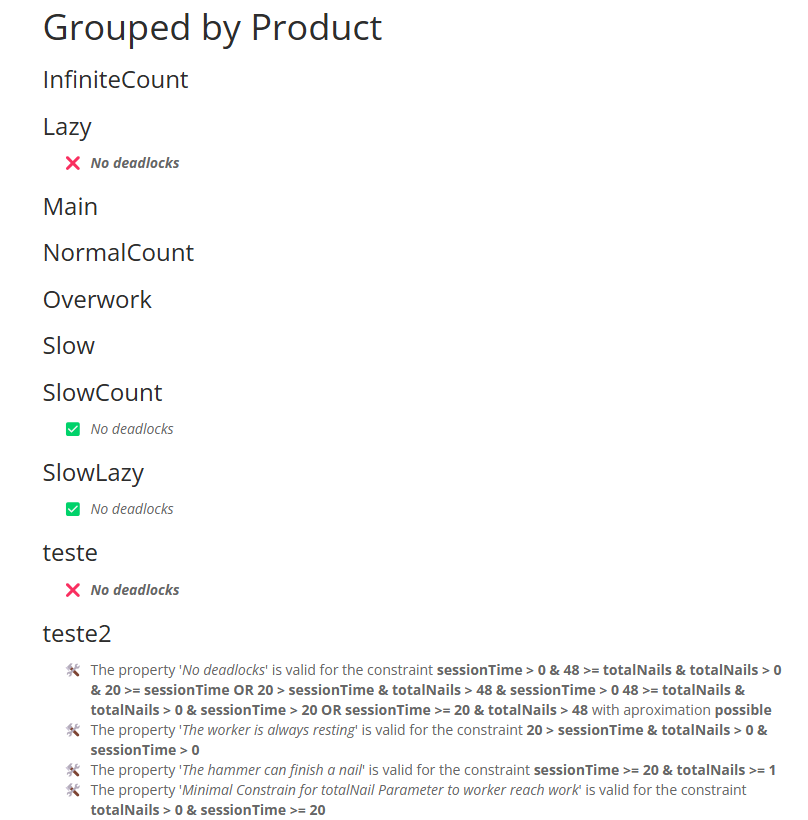
\includegraphics[width=\linewidth]{images/res2.png}};
            \begin{scope}[x={(image1.south east)},y={(image1.north west)}]
                \draw[black, thick] (0,0) rectangle (1,1); % coordenadas normalizadas
            \end{scope}
        \end{tikzpicture}
        \caption{Grouped by Product Report Result}
        \label{fig:GP}
    \end{minipage}
\end{figure}

\begin{figure}[H]
    \centering
    \begin{minipage}{\textwidth}
        \centering
        \begin{tikzpicture}
            \node[anchor=south west,inner sep=0] (image1) at (0,0) {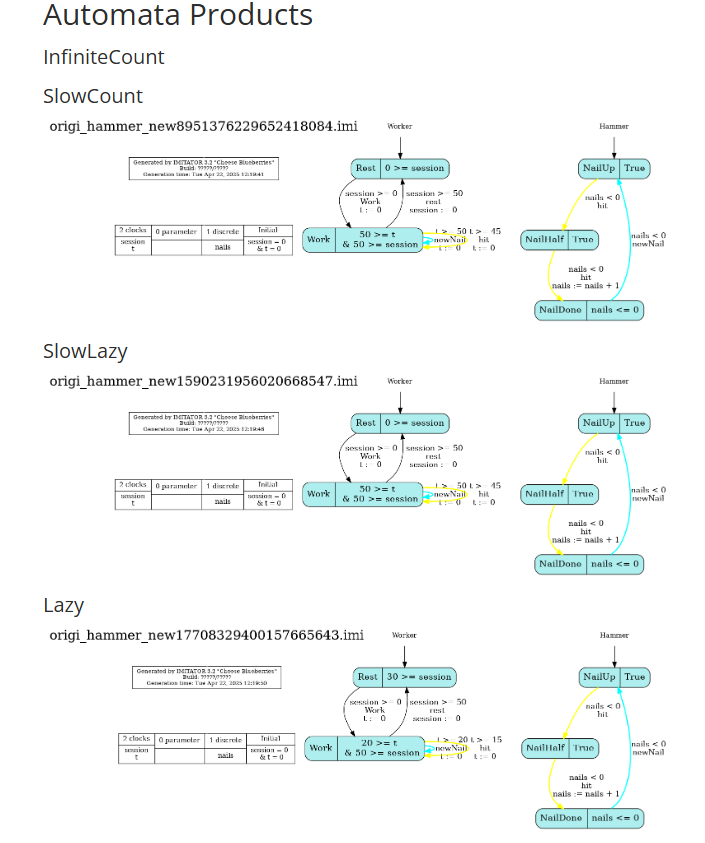
\includegraphics[width=\linewidth]{images/res3.png}};
            \begin{scope}[x={(image1.south east)},y={(image1.north west)}]
                \draw[black, thick] (0,0) rectangle (1,1); % coordenadas normalizadas
            \end{scope}
        \end{tikzpicture}
        \caption{Automata Products Part 1 Report Result}
        \label{fig:AP1}
    \end{minipage}
\end{figure}

\begin{figure}[H]
    \centering
    \begin{minipage}{\textwidth}
        \centering
        \begin{tikzpicture}
            \node[anchor=south west,inner sep=0] (image1) at (0,0) {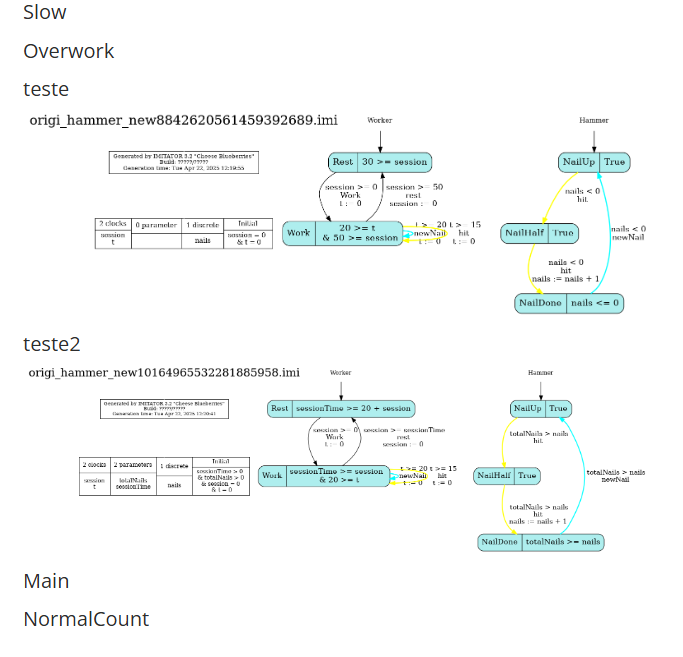
\includegraphics[width=\linewidth]{images/res4.png}};
            \begin{scope}[x={(image1.south east)},y={(image1.north west)}]
                \draw[black, thick] (0,0) rectangle (1,1); % coordenadas normalizadas
            \end{scope}
        \end{tikzpicture}
        \caption{Automata Products Part 2 Report Result}
        \label{fig:AP2}
    \end{minipage}
\end{figure}





